\documentclass[10pt]{article}
\usepackage[document]{ragged2e}
\usepackage{multicol}
\usepackage[margin=1in]{geometry}
\usepackage{titlesec}
\usepackage{fancyhdr}
\usepackage{graphicx}
\graphicspath{ {./images/} }
\usepackage[justification=centering]{caption}
\captionsetup[subfigure]{justification=centering}
\captionsetup[figure]{justification=centering}
\usepackage{subcaption}
\usepackage{float}


\pagestyle{fancy}
\fancyhf{}
\fancyfoot[R]{Page. \thepage}
\fancypagestyle{plain}{
    \renewcommand{\headrulewidth}{0pt}
    \fancyhf{}
    \fancyfoot[R]{Page. \thepage}
}

\setlength{\parindent}{0em}
\setlength{\parskip}{1em}
\titlespacing*{\section}{0pt}{0.2em}{0.5em}
\titlespacing*{\subsection}{0pt}{0.2em}{0.2em}
\titlespacing*{\subsubsection}{0pt}{0.2em}{0.2em}


\title{Final Report}
\author{The Freedom Deer: Tianchang Li, Hualiang Qin, Qingwei Lan}

\begin{document}
\maketitle


\begin{figure}[H]
\captionsetup{font=small}
    \begin{subfigure}{0.5\textwidth}
        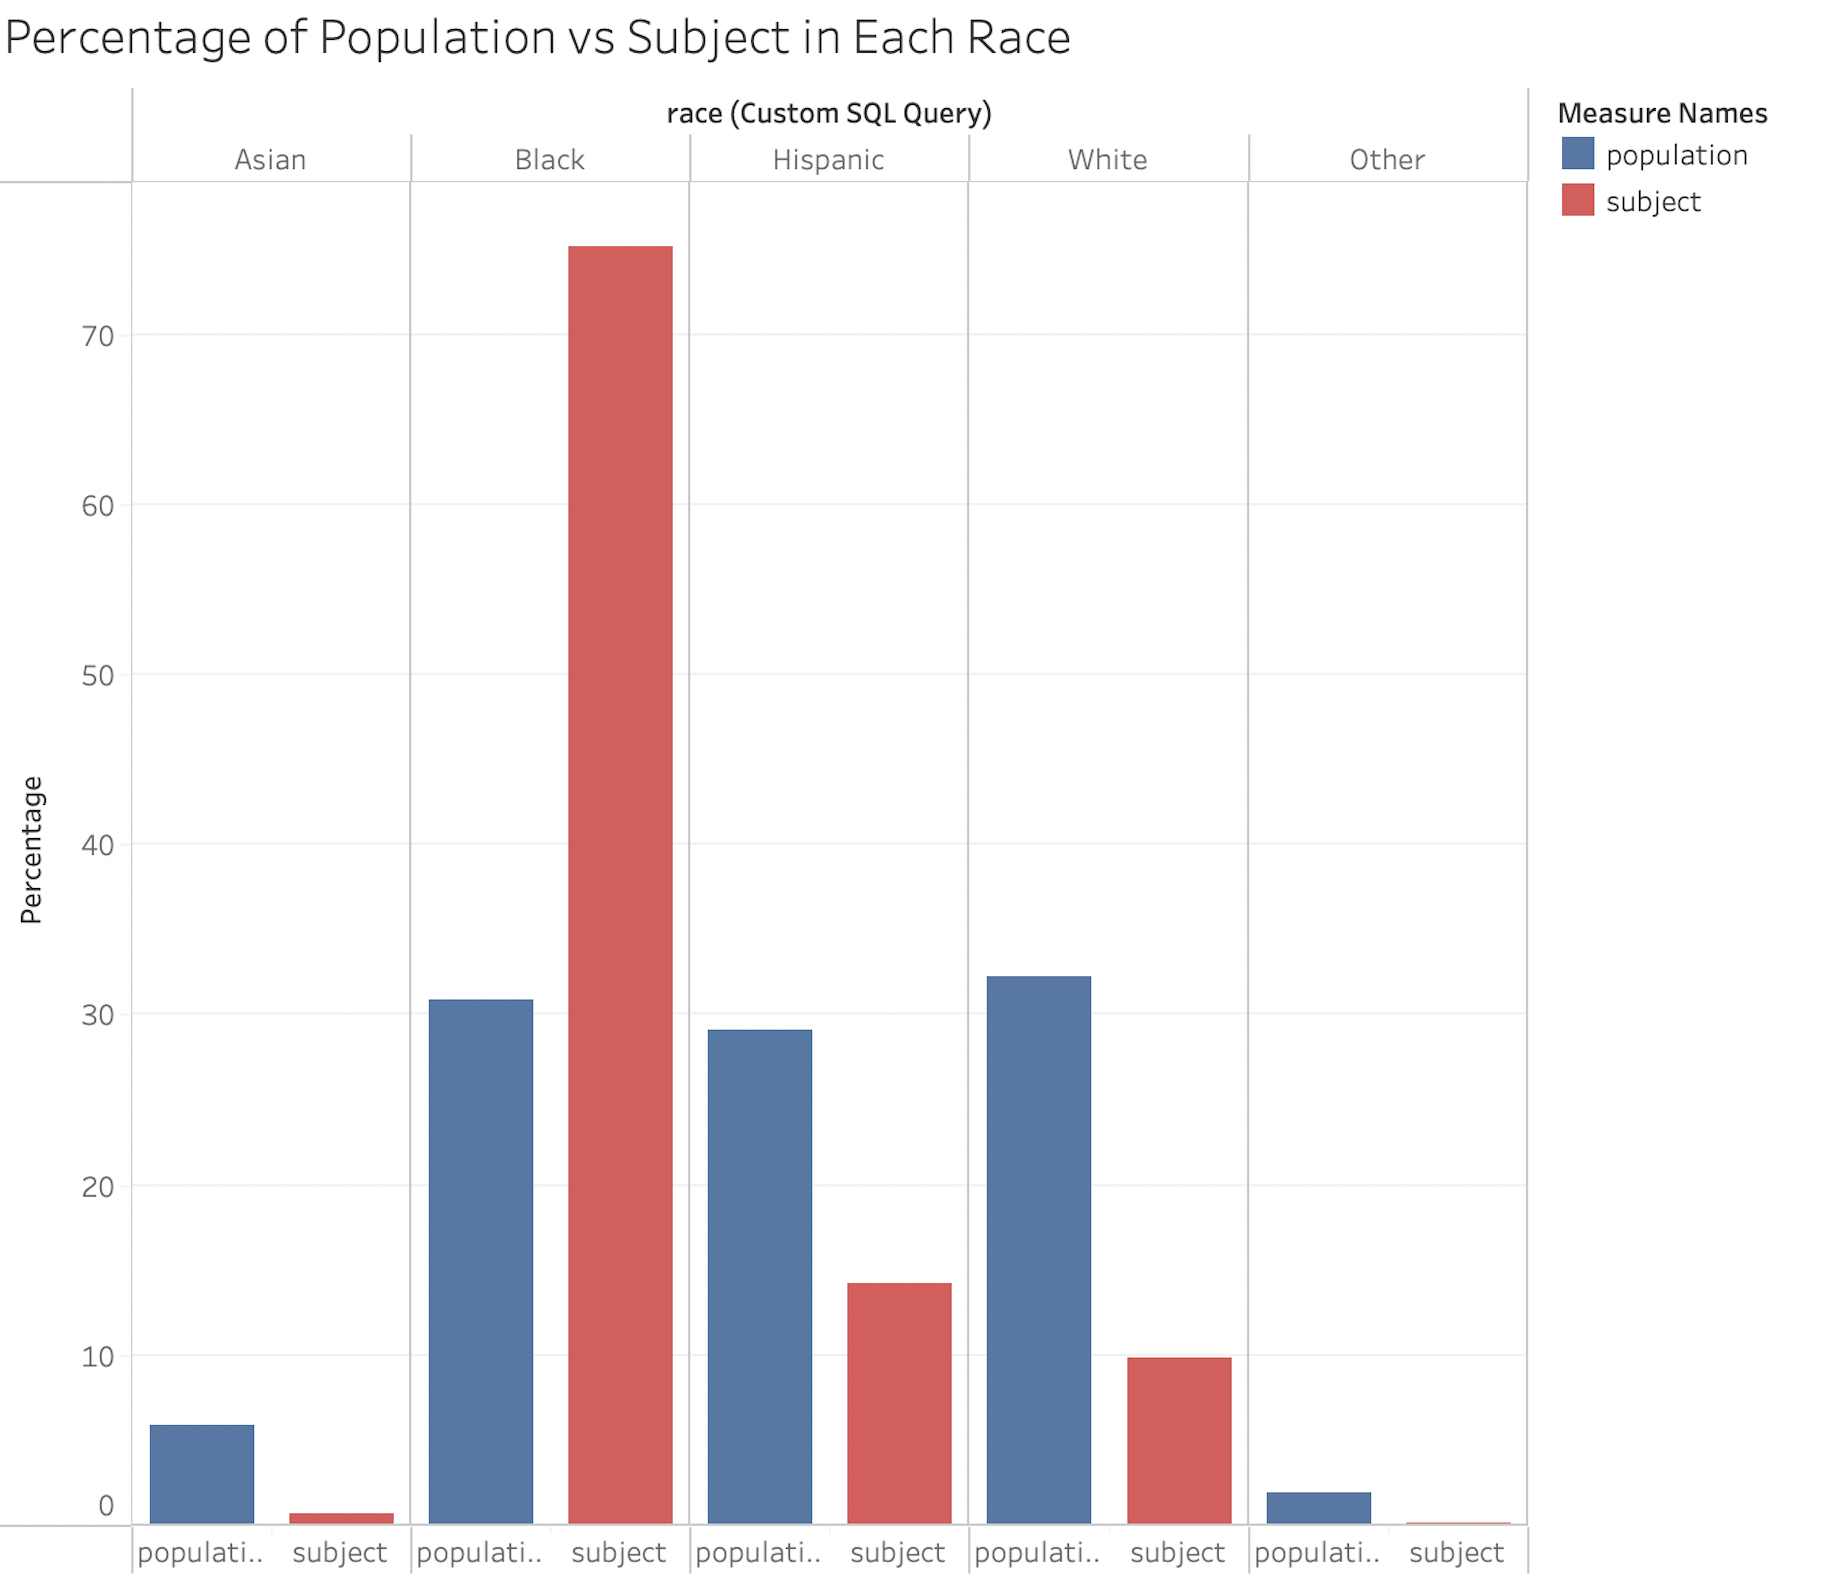
\includegraphics[width=\textwidth]{img1}
        \caption{Barcharts of (1) the percentage of the population of each race compared to the total population and (2) the percentage of use of force cases on subjects of each race compared to total use of force cases}
        \label{img1}
    \end{subfigure}%
    \begin{subfigure}{0.5\textwidth}
        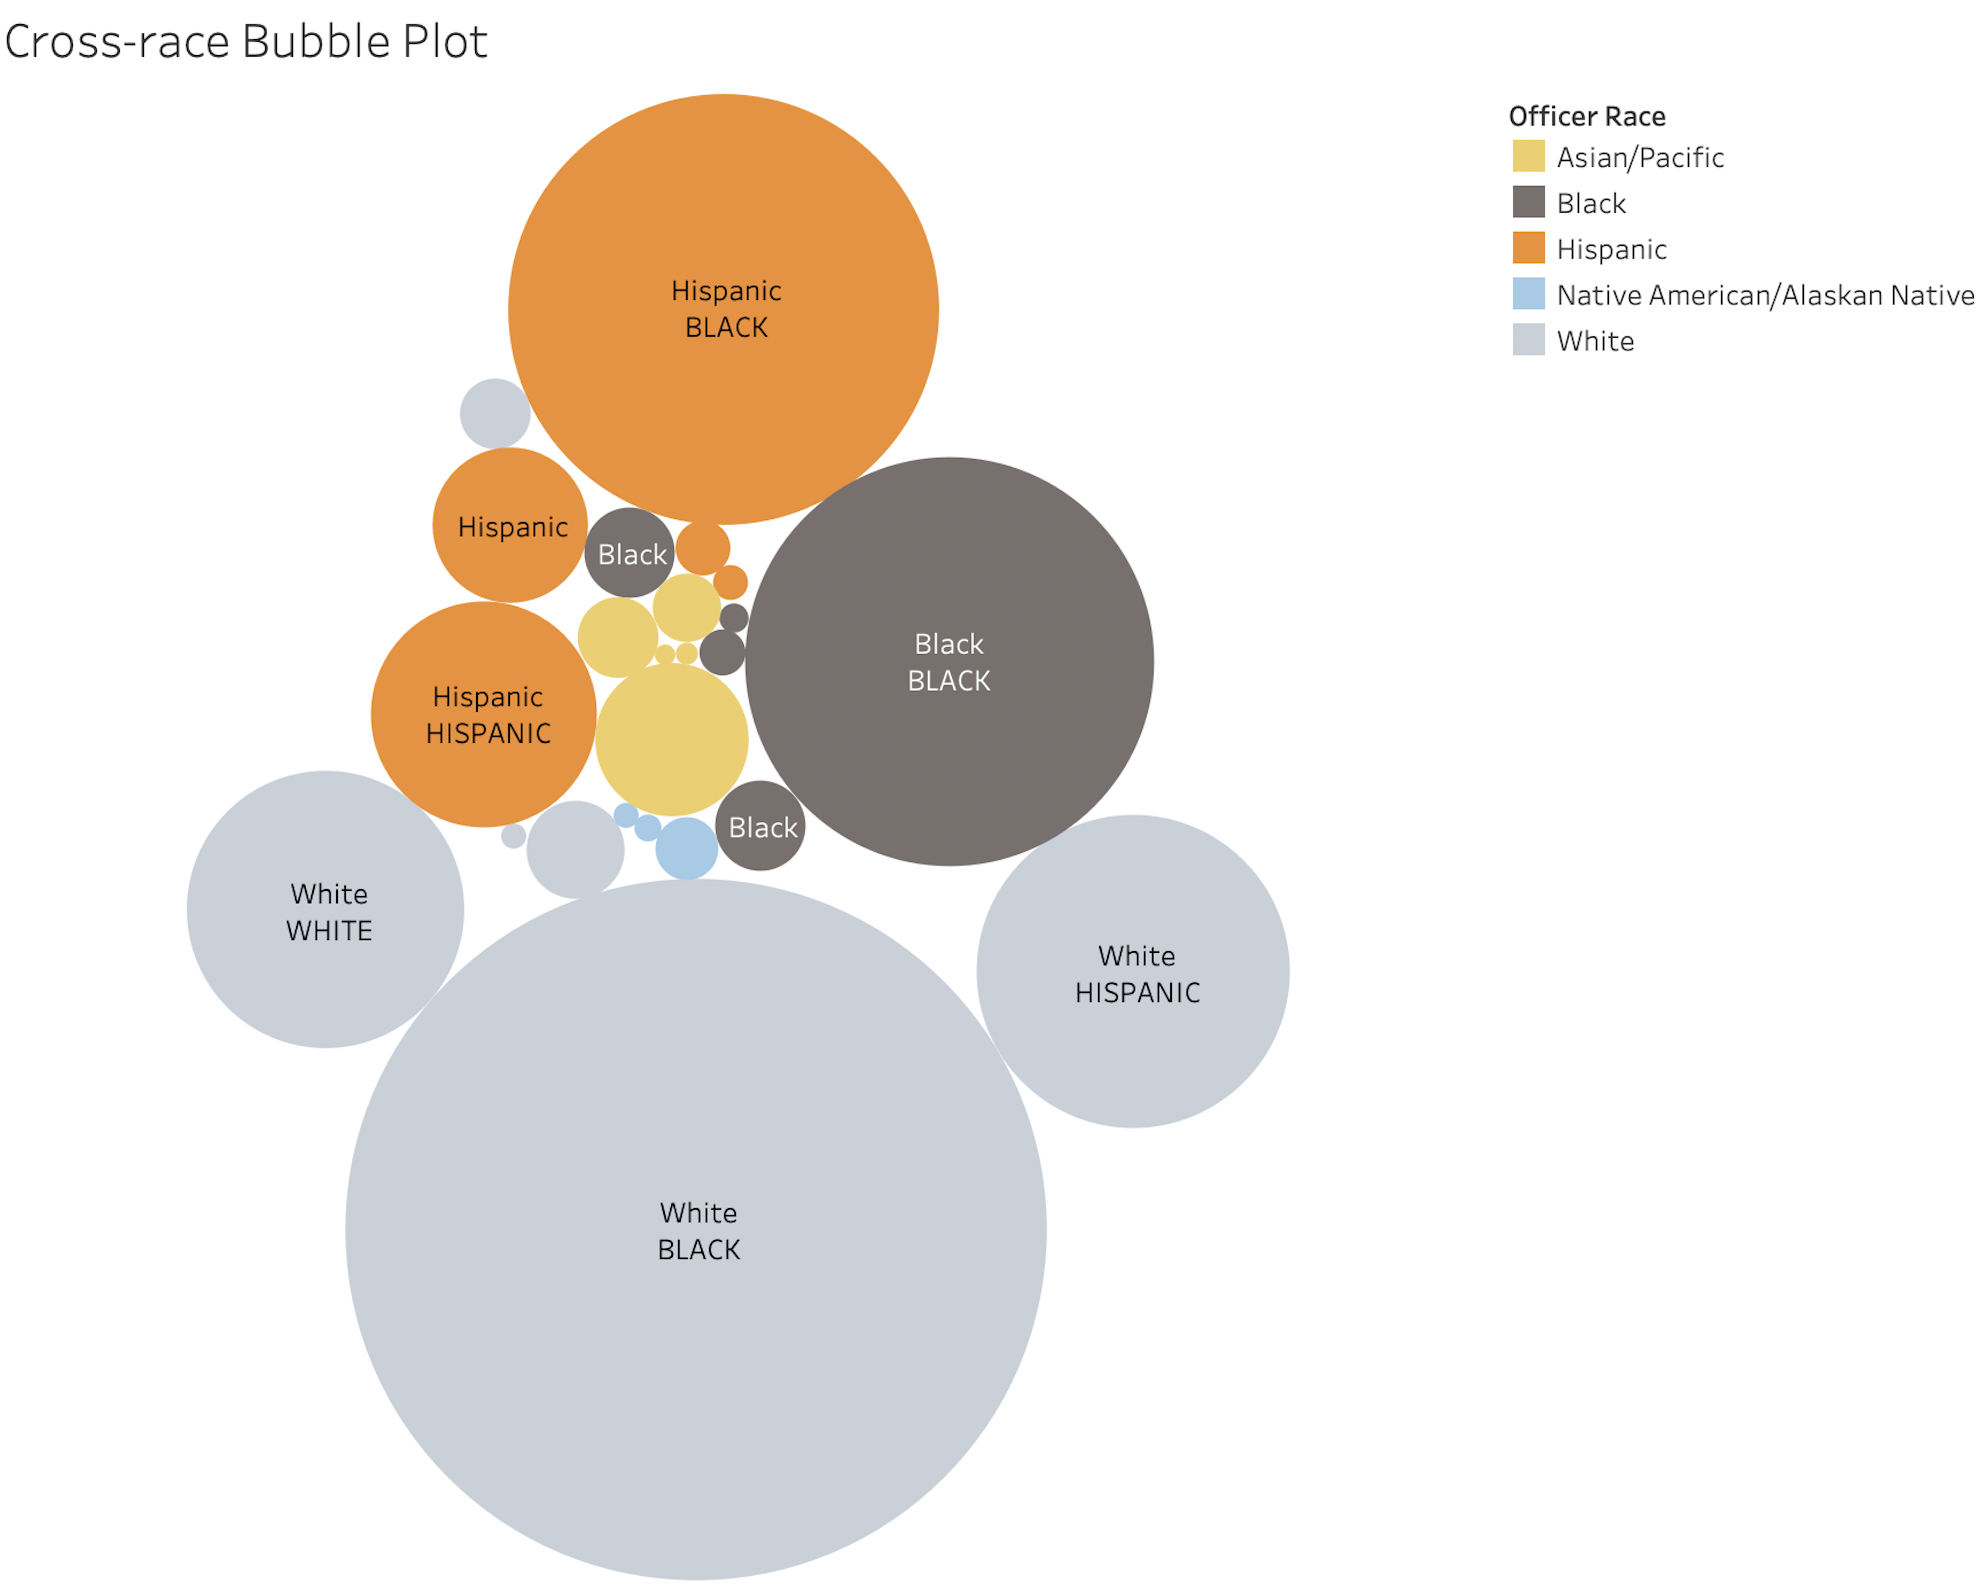
\includegraphics[width=\textwidth]{img3}
        \caption{Bubble plot depicting cross-race use of force cases}
        \label{img3}
    \end{subfigure}
\caption{Racial composition graphs}
\end{figure}


\begin{figure}[H]
\centering
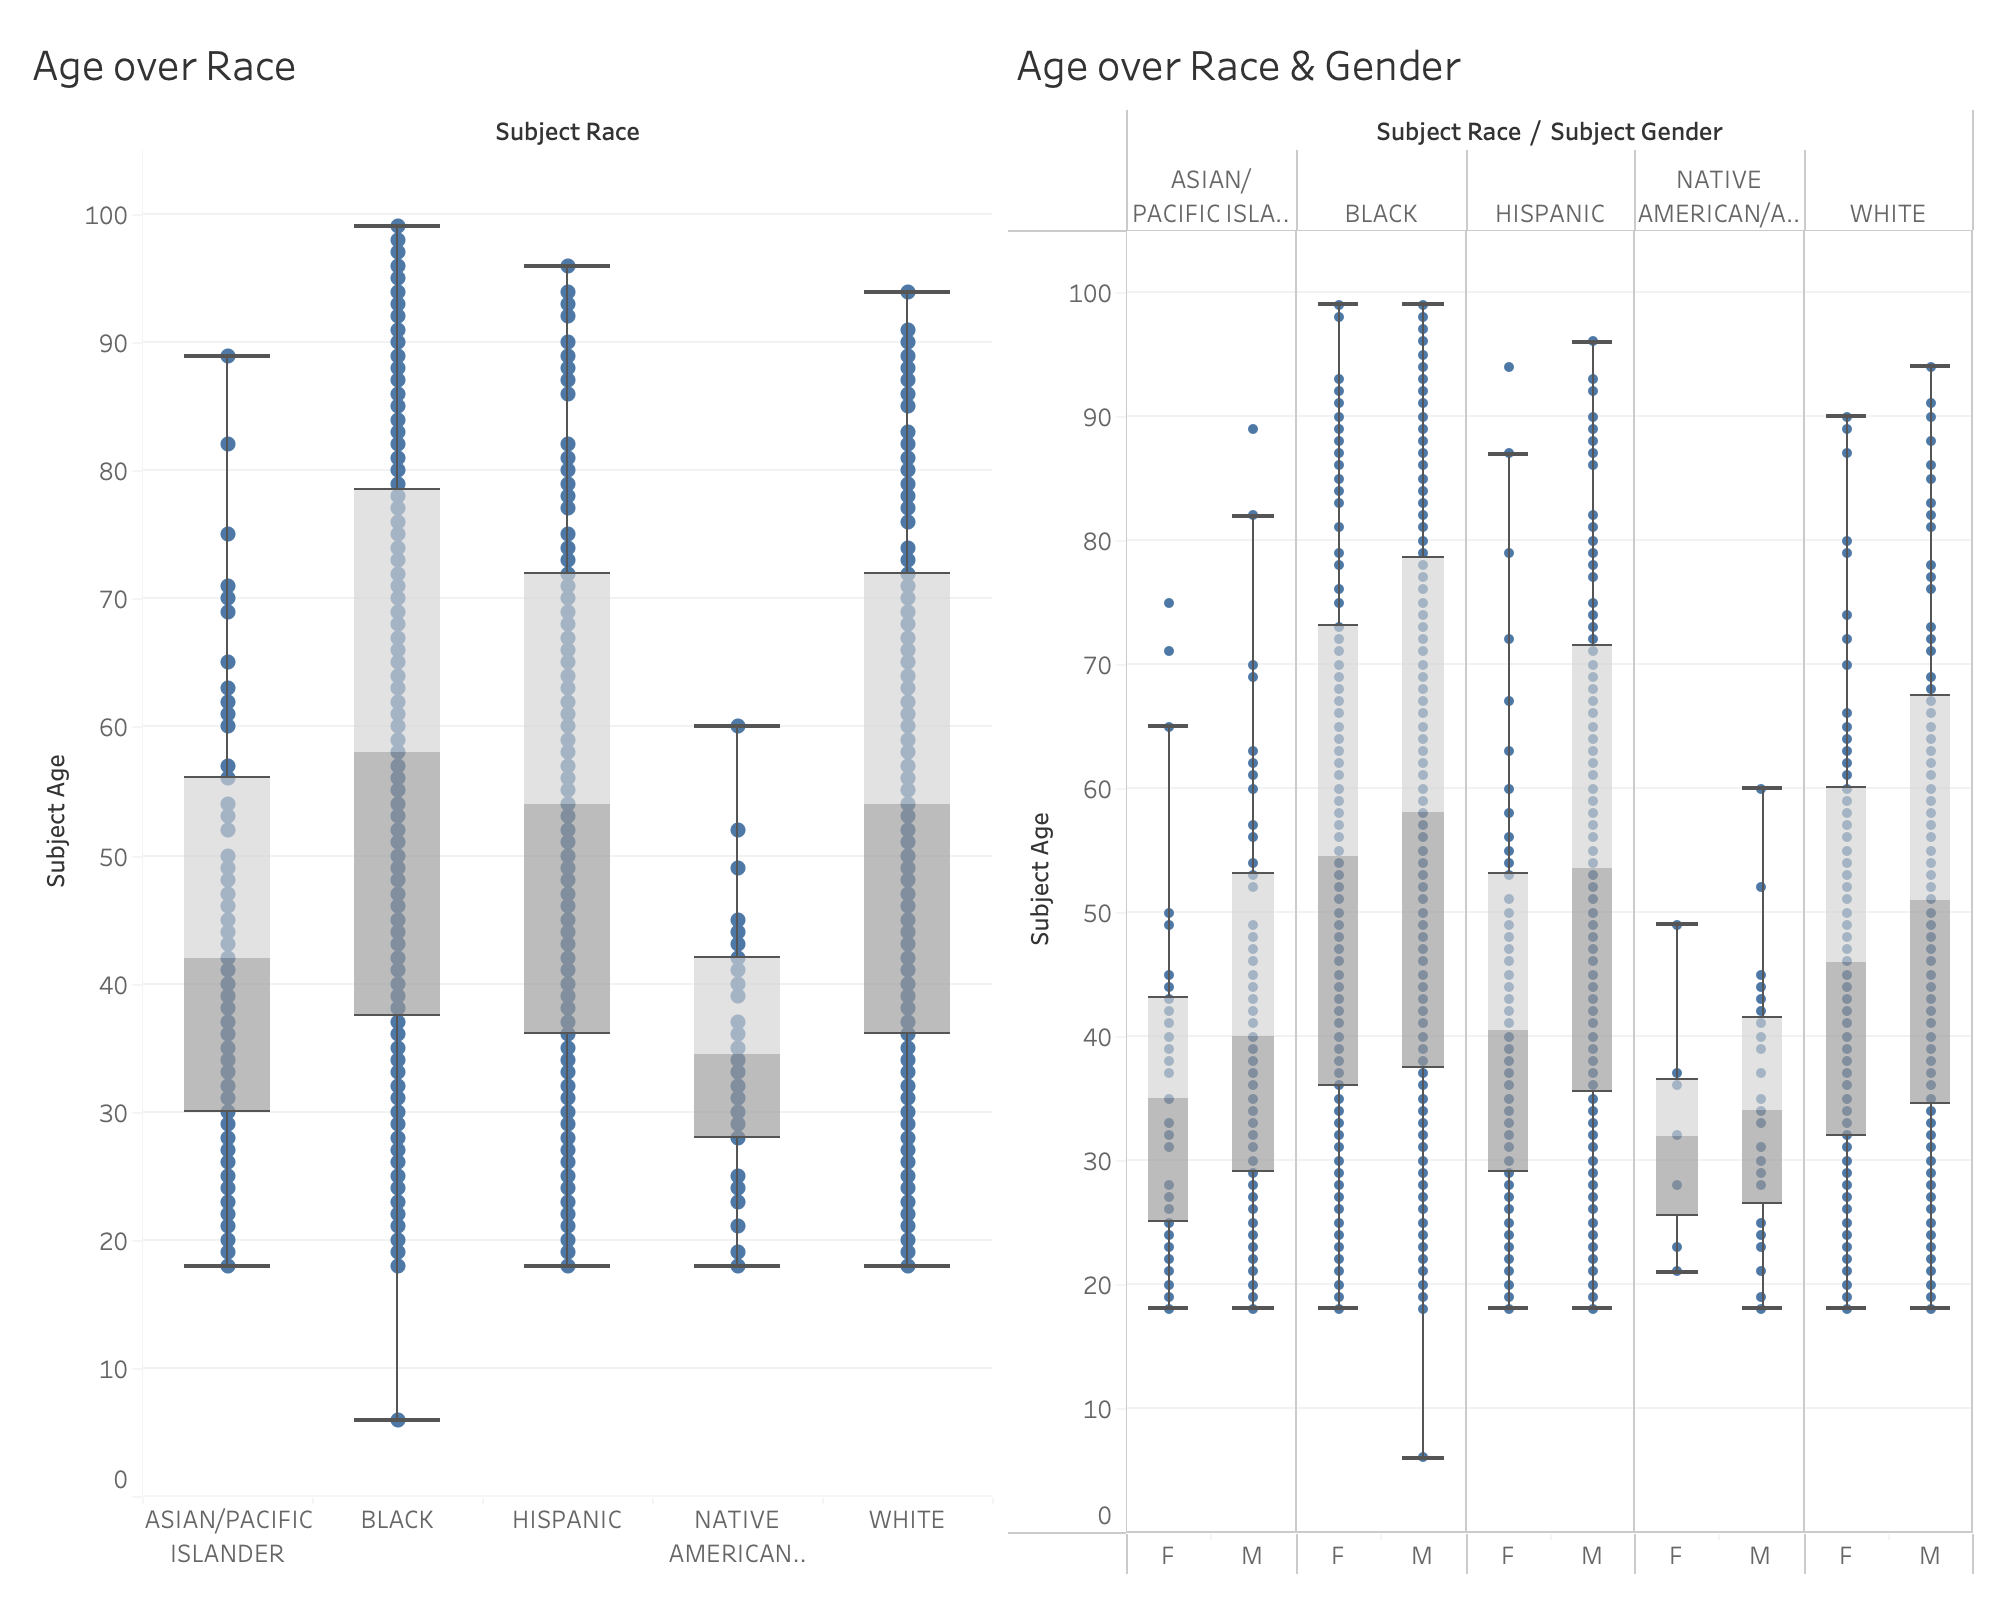
\includegraphics[width=0.8\textwidth]{img2}
\caption{Box and whisker plot of subject age over race and gender}
\label{img2}
\end{figure}


\begin{figure}[H]
\captionsetup{font=small}
    \begin{subfigure}{0.5\textwidth}
        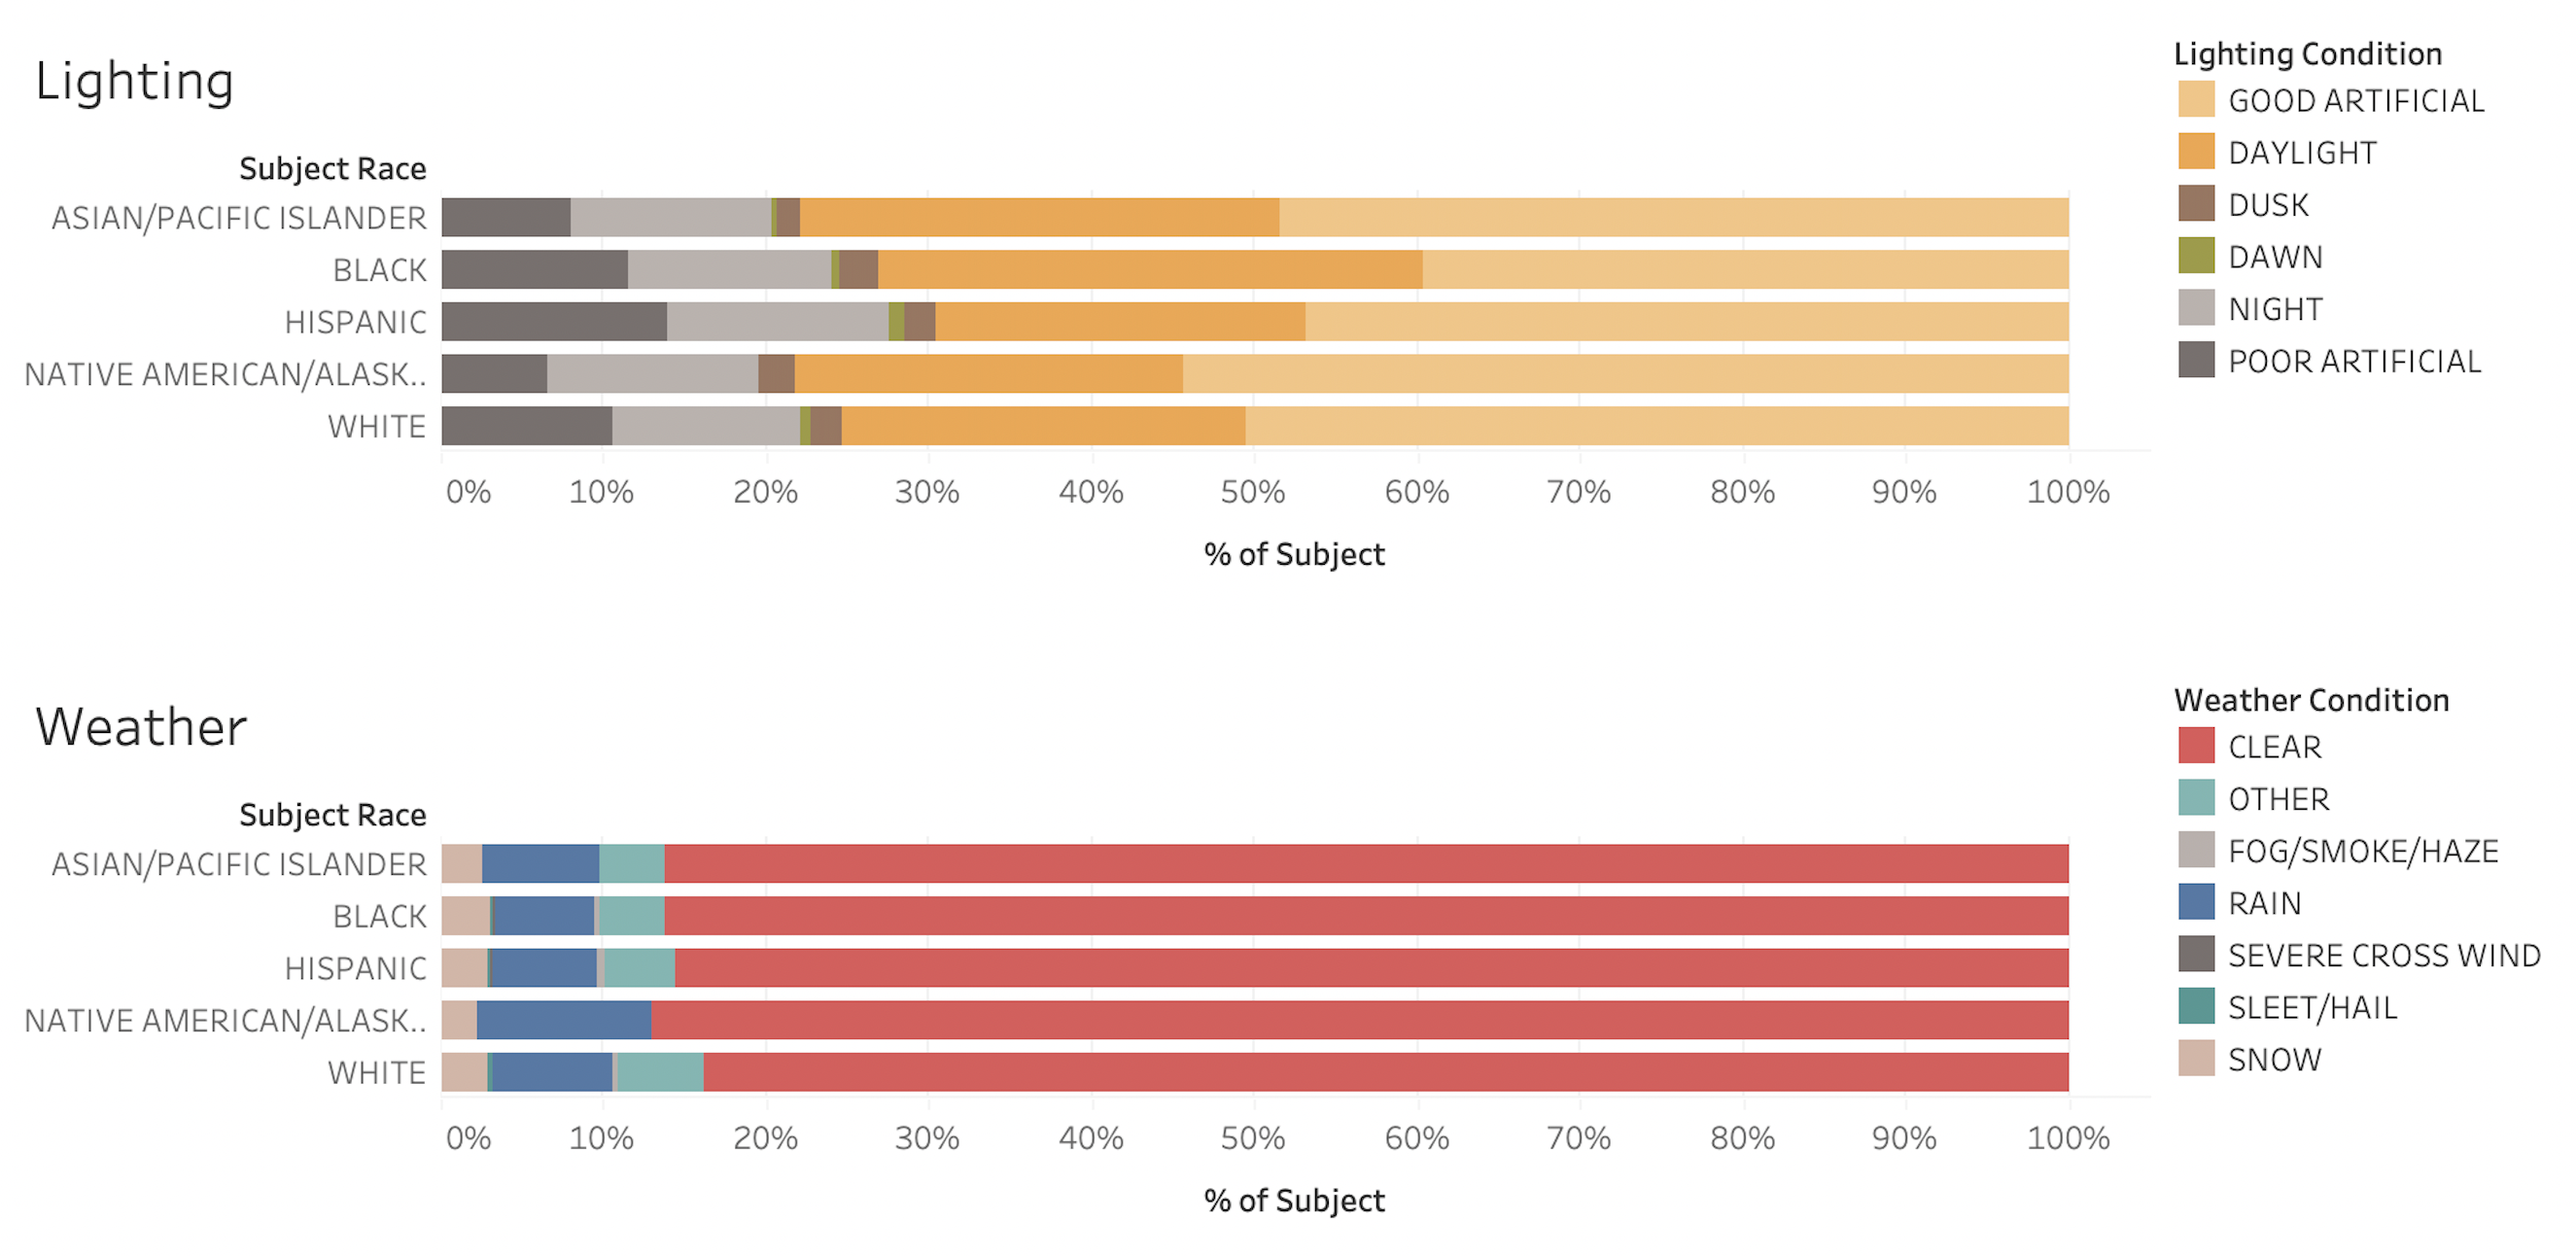
\includegraphics[width=\textwidth]{img4}
        \label{img4}
    \end{subfigure}%
    \begin{subfigure}{0.5\textwidth}
        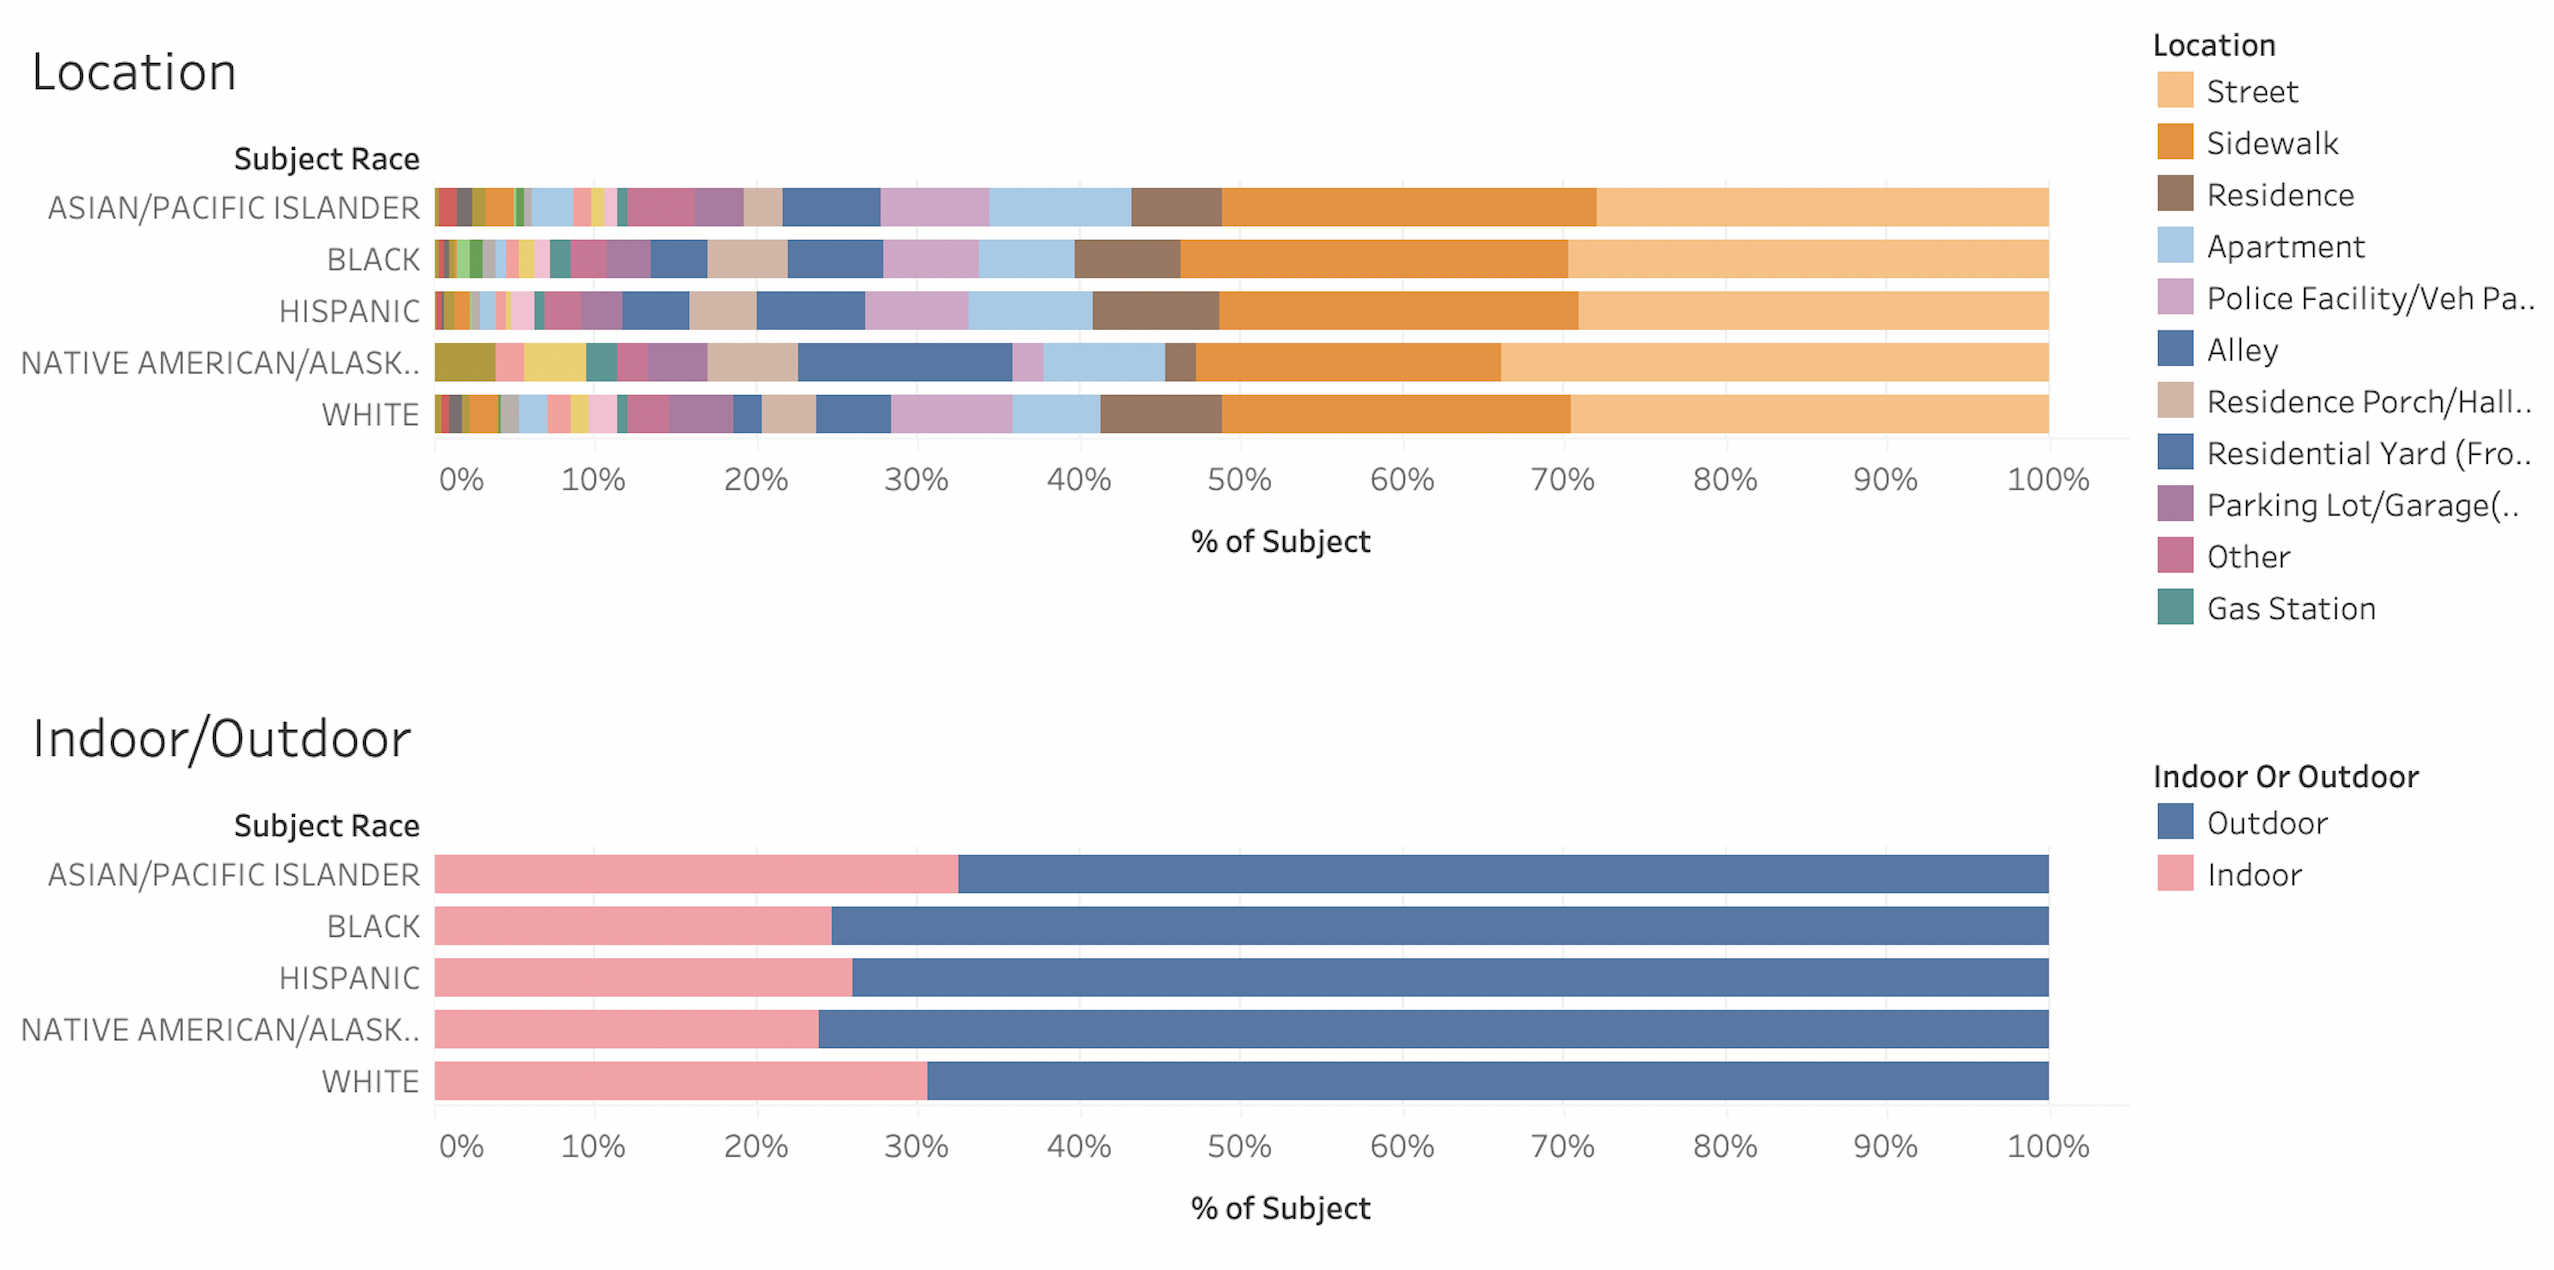
\includegraphics[width=\textwidth]{img5}
        \label{img5}
    \end{subfigure}
\label{barcharts}
\caption{Barcharts of the frequency of police use of force cases in different environmental conditions (lighting, weather, location, indoors/outdoors) over each race}
\end{figure}


\begin{figure}[H]
\captionsetup{font=small}
    \begin{subfigure}{0.5\textwidth}
        \frame{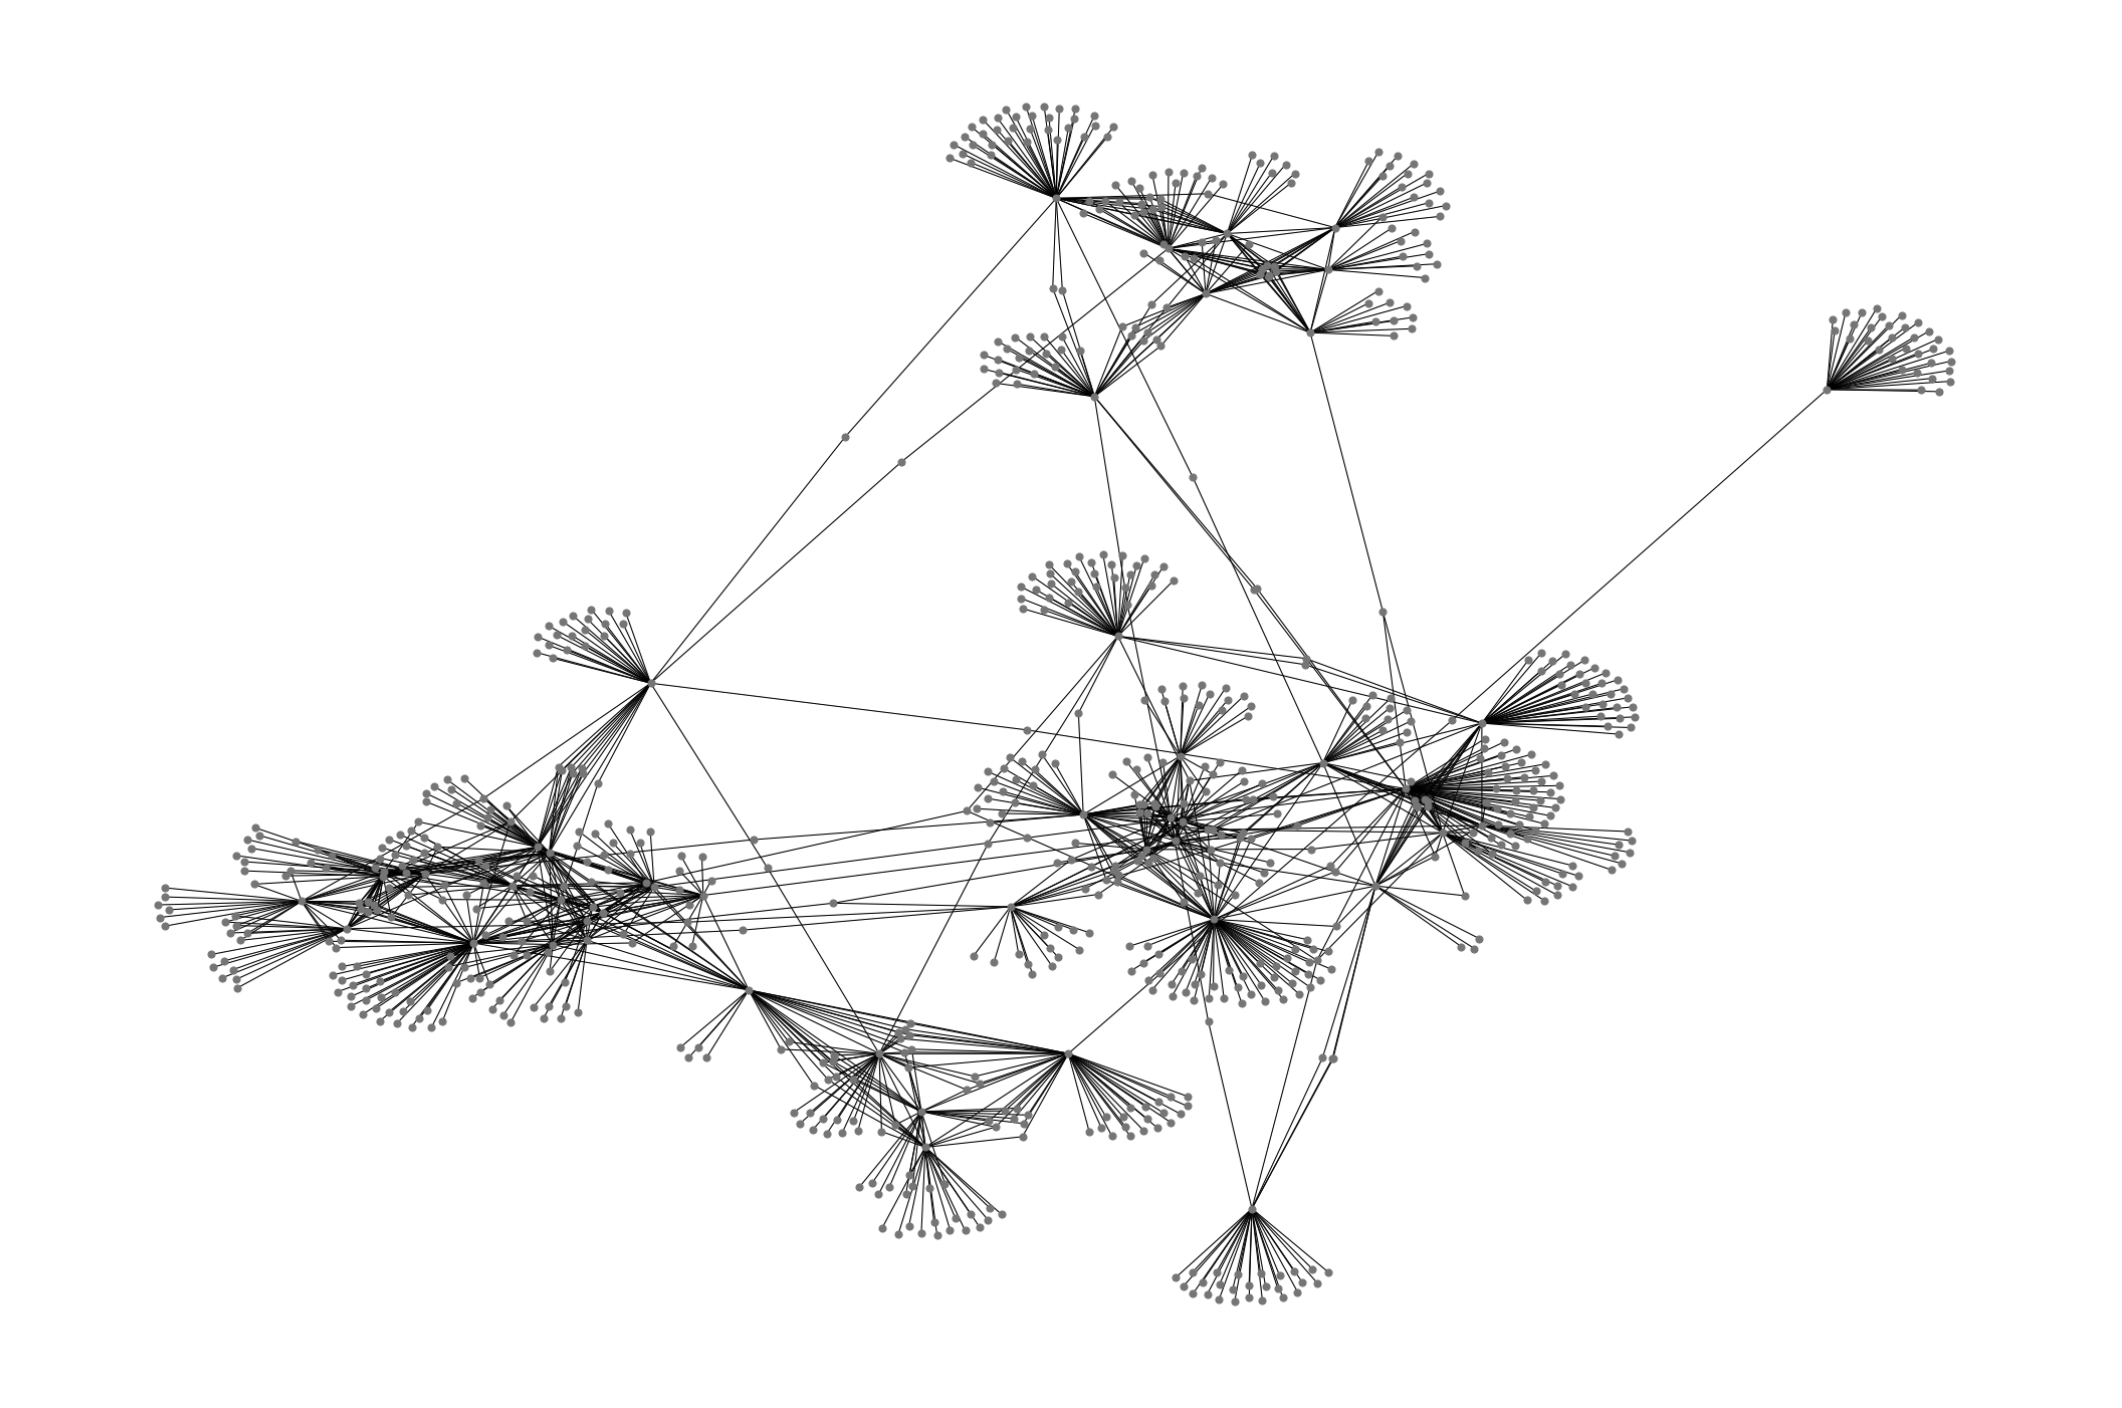
\includegraphics[width=\textwidth]{trr}}
        \caption{TRR network graph}
        \label{trr}
    \end{subfigure}%
    \begin{subfigure}{0.5\textwidth}
        \frame{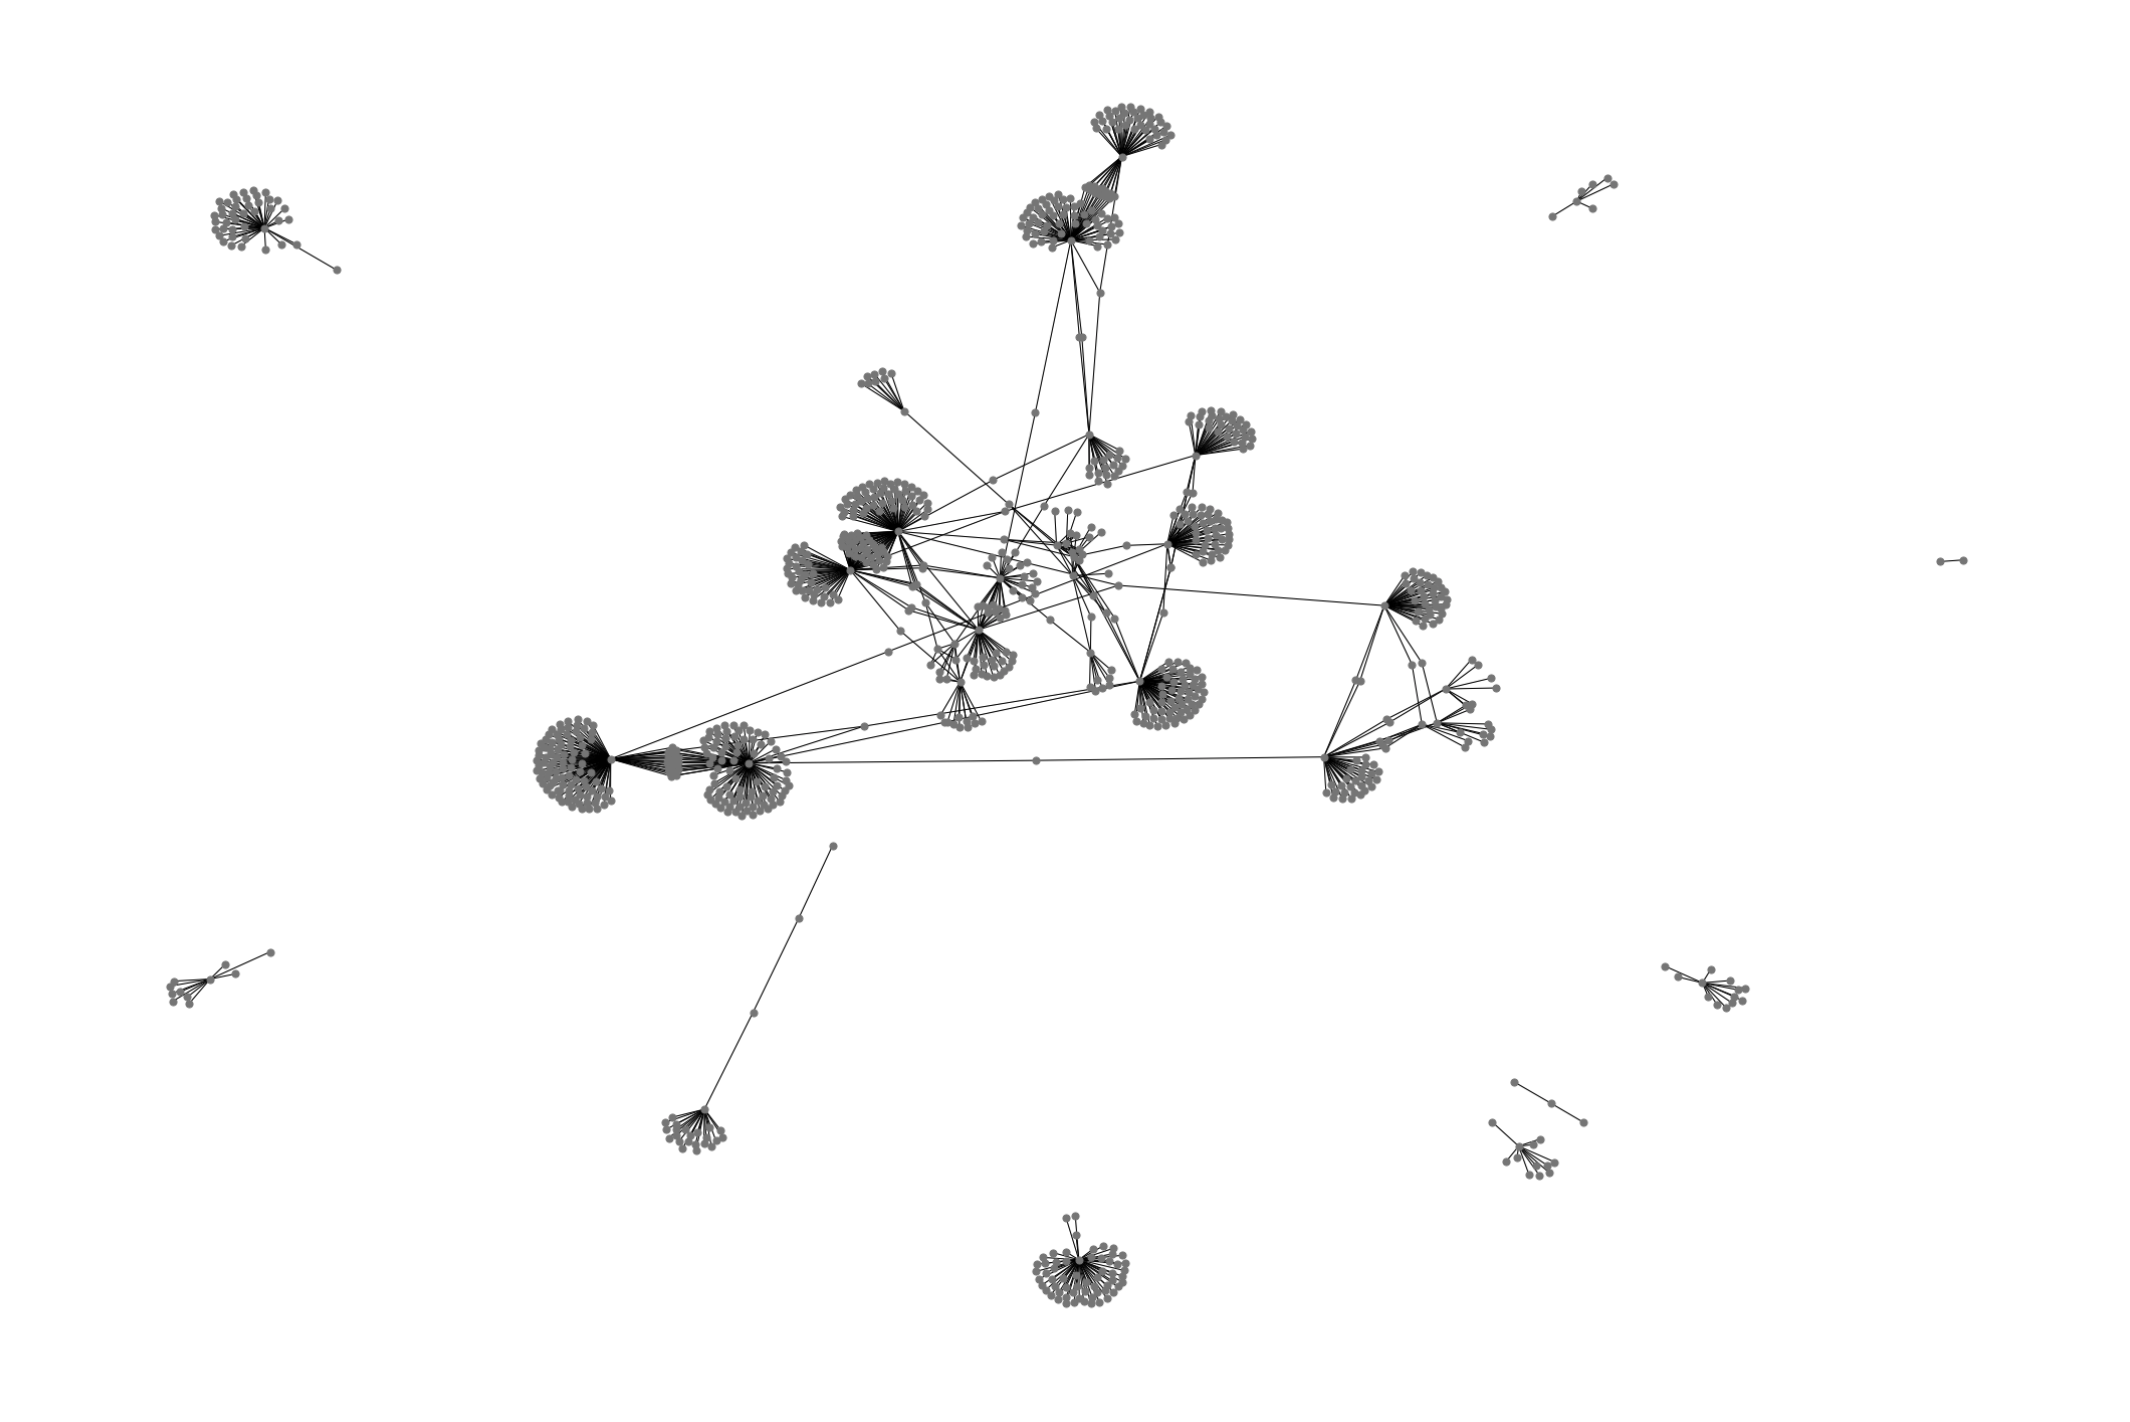
\includegraphics[width=\textwidth]{baseline}}
        \caption{Baseline network graph}
        \label{baseline}
    \end{subfigure}
\caption{TRR network graph and baseline network graph for all TRR cases.}
\end{figure}


\begin{figure}[H]
\captionsetup{font=small}
    \begin{subfigure}{0.5\textwidth}
        \frame{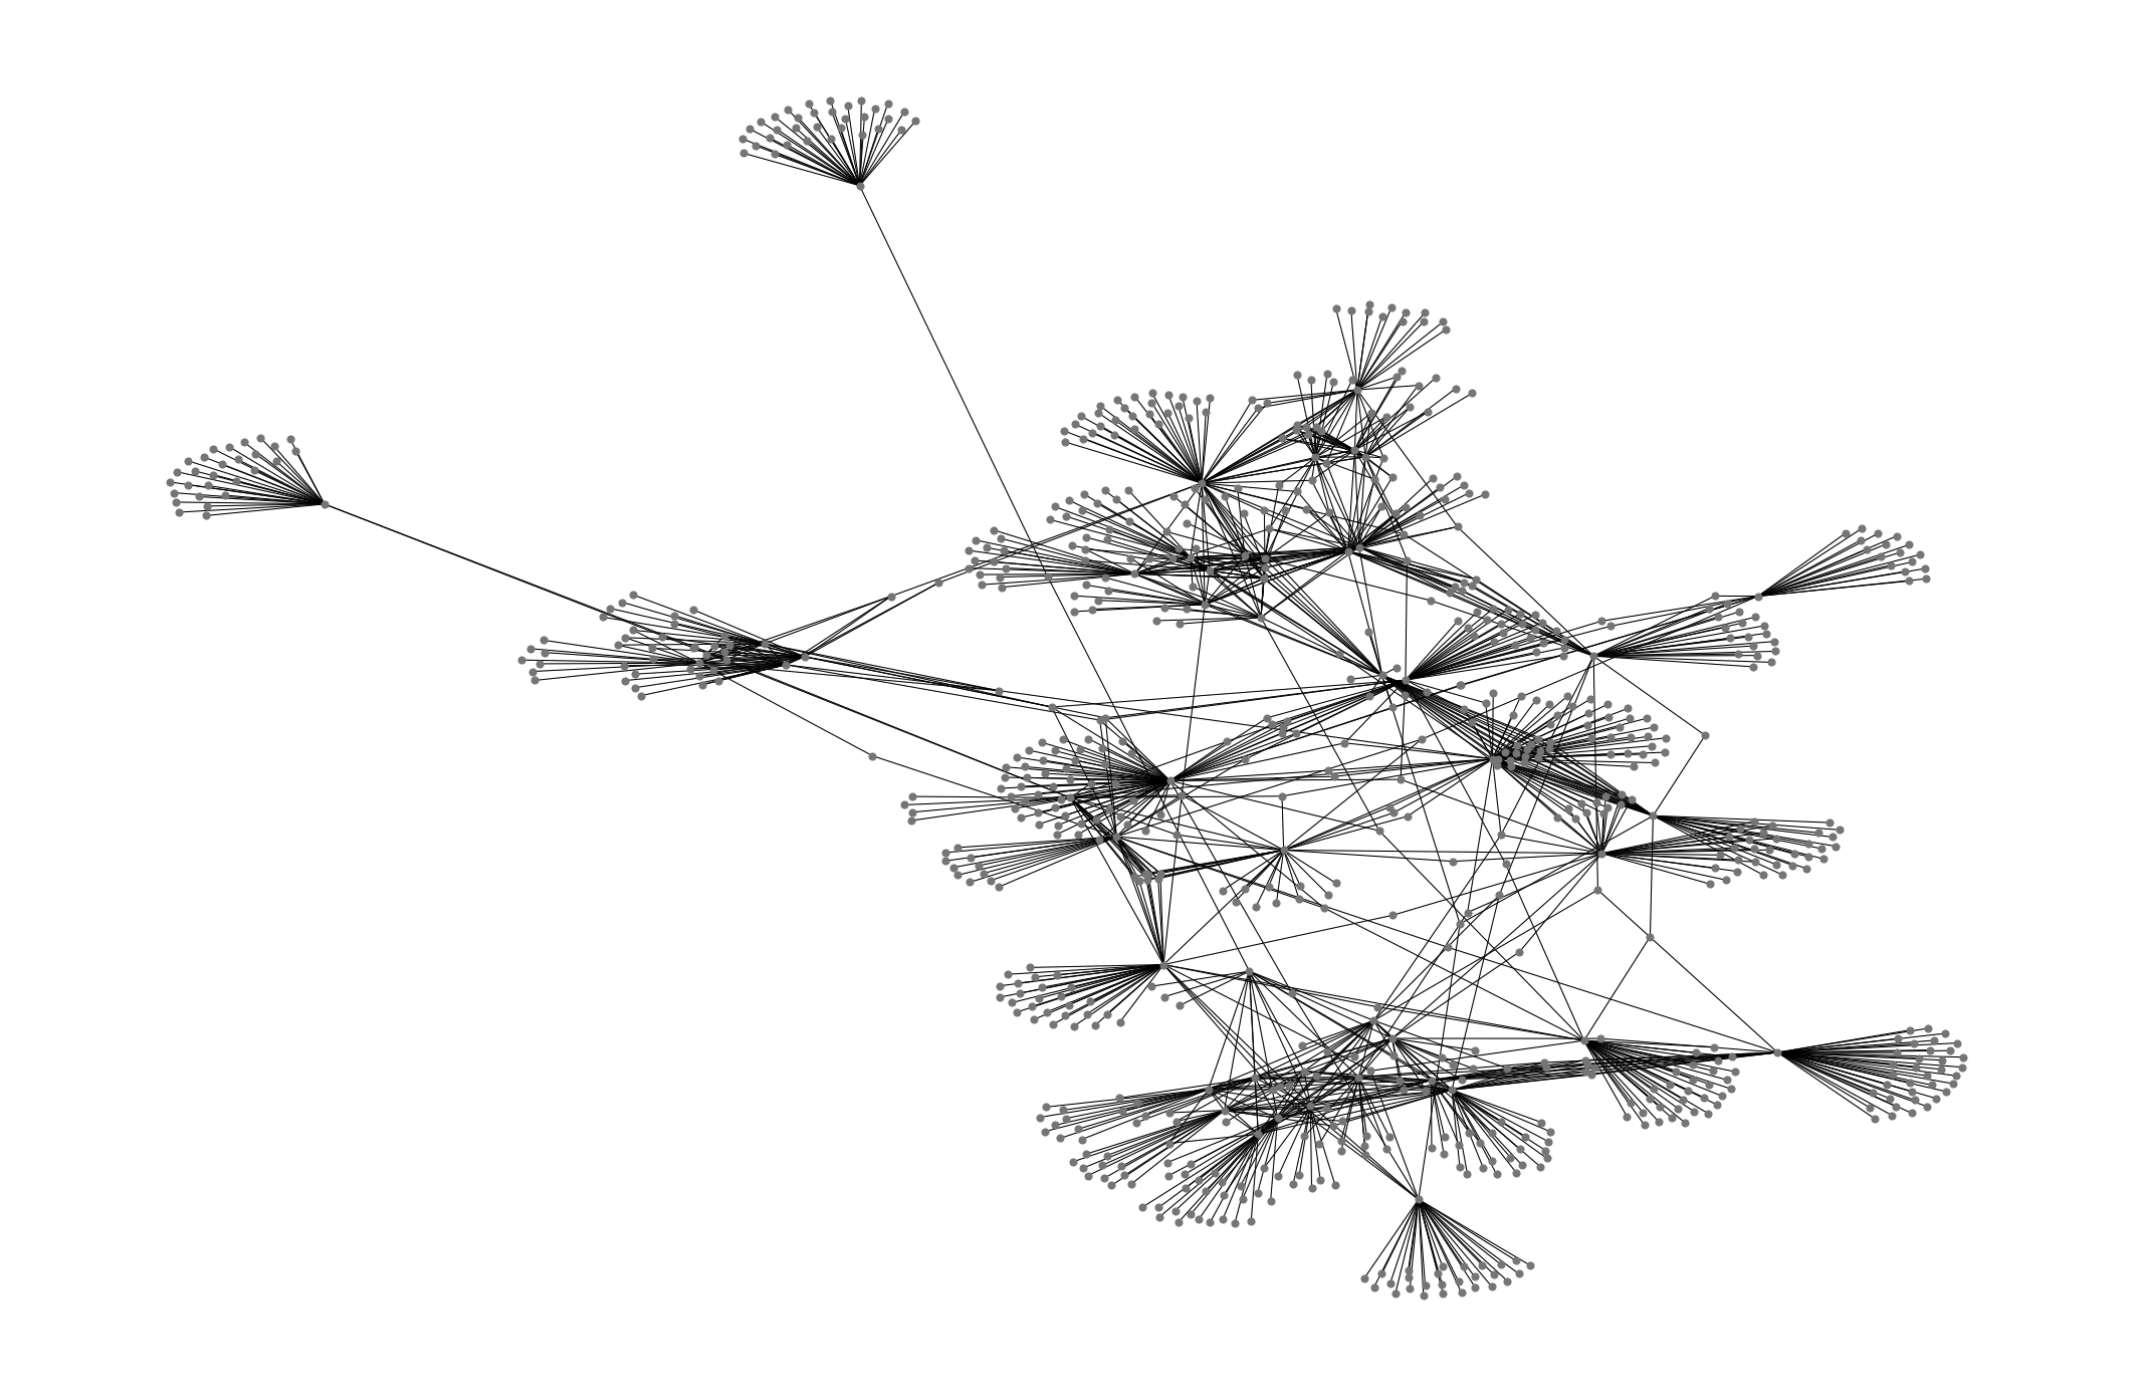
\includegraphics[width=\textwidth]{trr_cross_race}}
        \caption{TRR network graph}
        \label{trr_cross_race}
    \end{subfigure}%
    \begin{subfigure}{0.5\textwidth}
        \frame{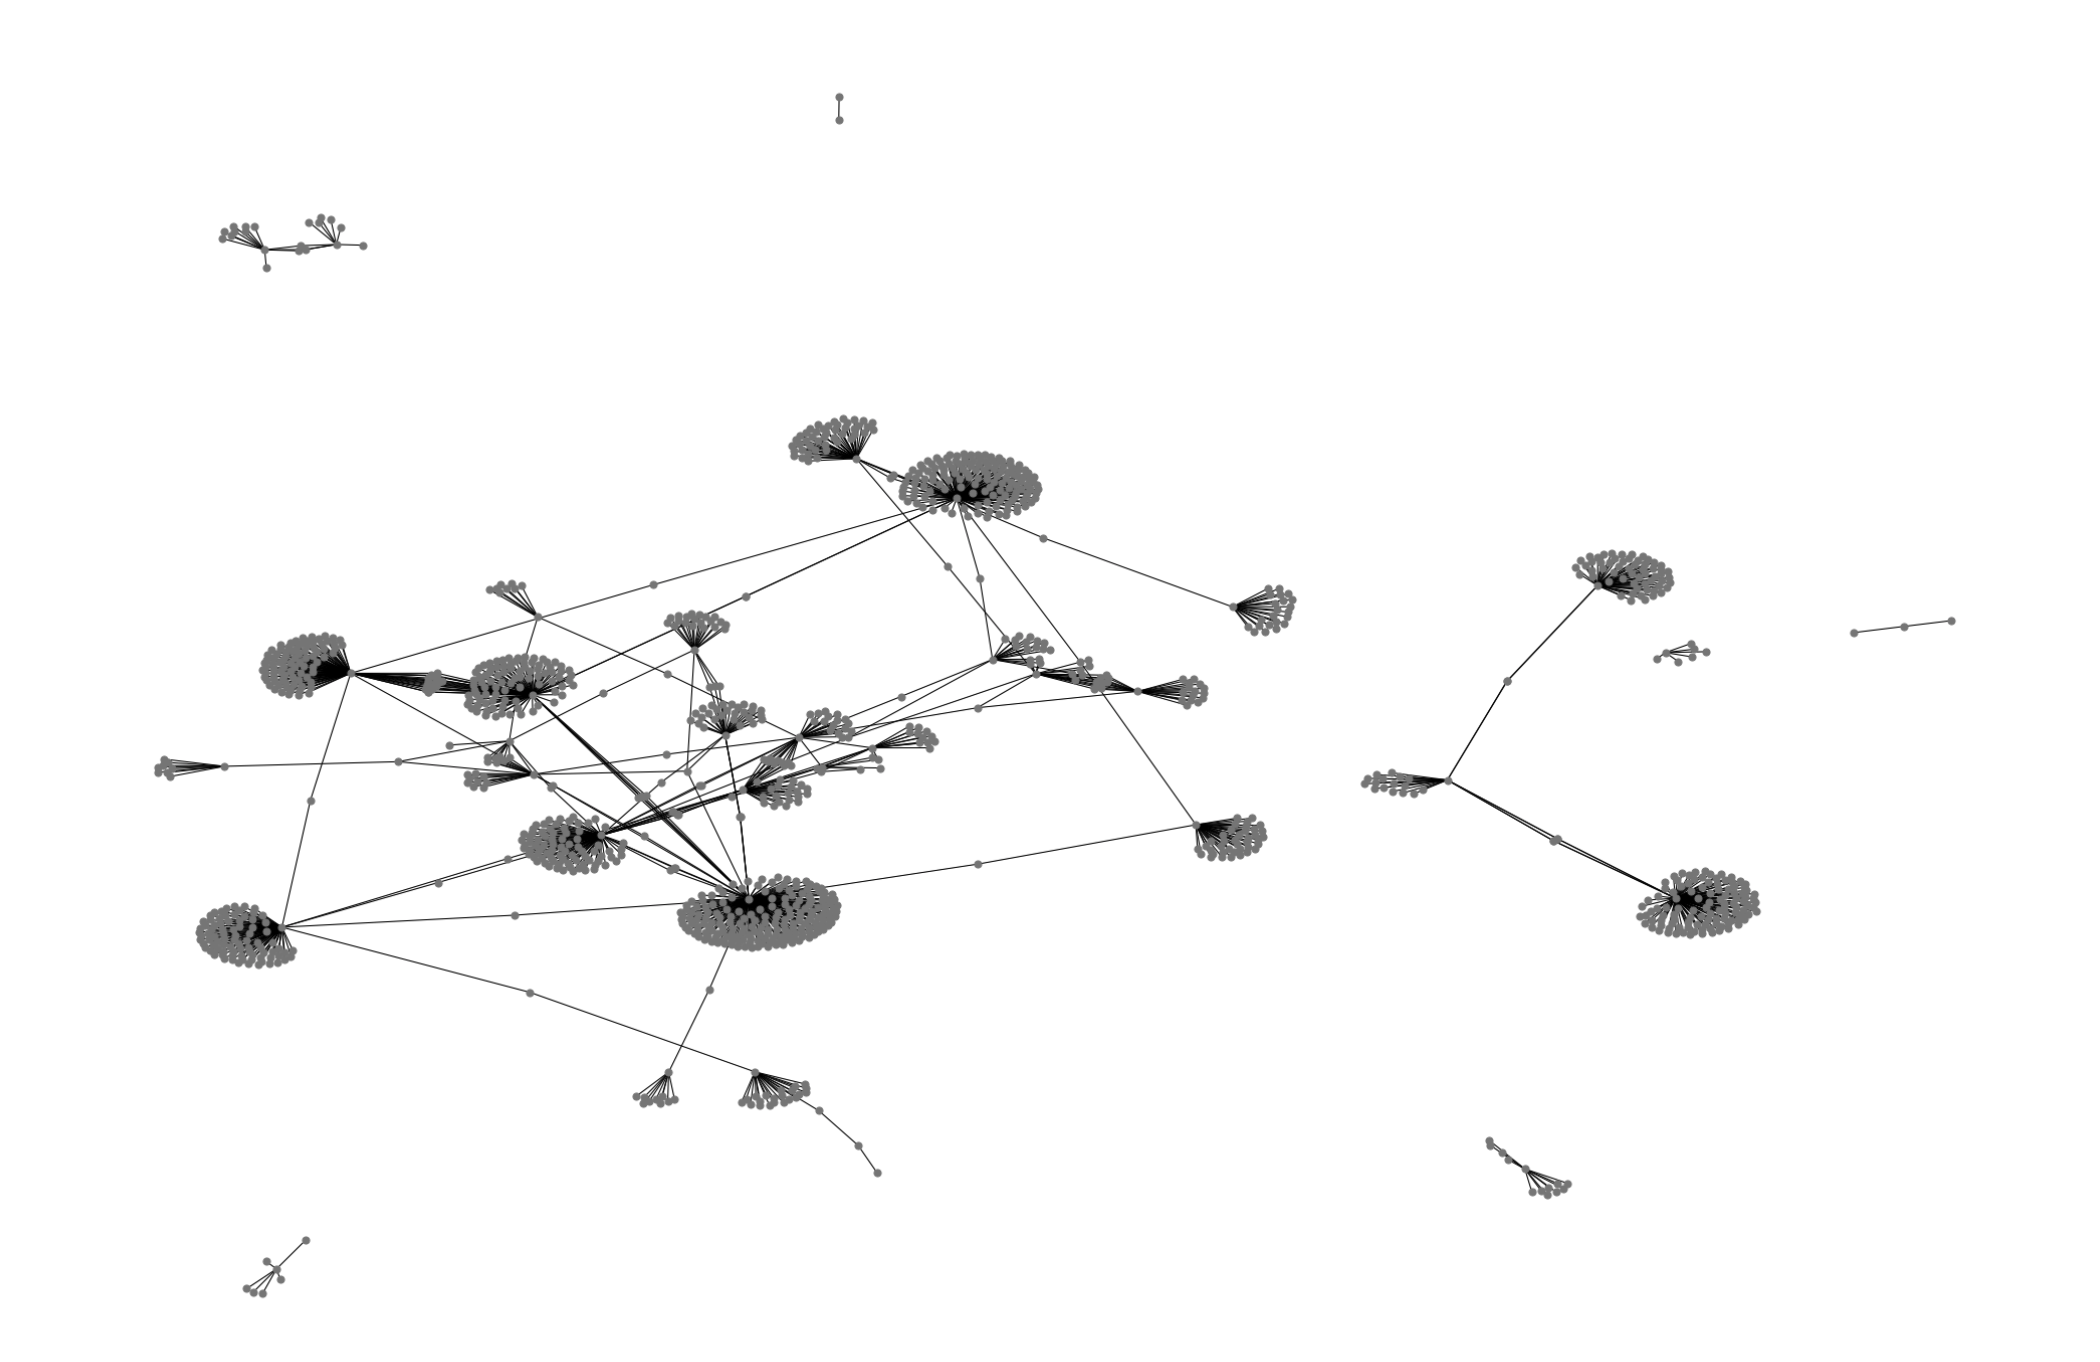
\includegraphics[width=\textwidth]{baseline_cross_race}}
        \caption{Baseline network graph}
        \label{baseline_cross_race}
    \end{subfigure}
\caption{TRR network graph and baseline network graph for TRR cases involving only \textbf{cross-race use of force}.}
\end{figure}



\end{document}
